
\section{Leitungstheorie}

\subsection{Leitungsgleichungen}
	\begin{tabular}{p{8cm}p{4.5cm}p{5cm}}
		\begin{minipage}{8cm}
	    	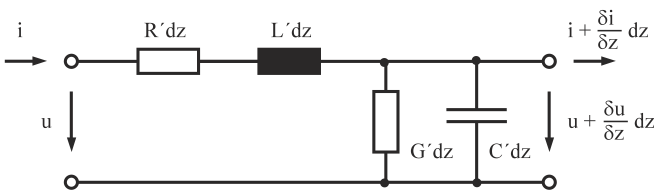
\includegraphics[width=8cm]{/bilder/LeitungselementESB.png}
	    \end{minipage}&
		\begin{minipage}{4.5cm}
	    	\textbf{Leitungsbeläge}\\
	    	$R'[\frac{\Omega}{m}]: \text{Widerstandsbelag}$\\
	    	$L'[\frac{H}{m}]: \text{Induktivitätsbelag}$\\
	    	$G'[\frac{S}{m}]: \text{Leitwertbelag}$\\
	    	$C'[\frac{F}{m}]: \text{Kapazitätsbelag}$\\
	    \end{minipage}&
		\begin{minipage}{5cm}
        	\textbf{Leerlauf}:\\
        		$\underline{Y}_L=\frac{1}{\underline{Z}_L}=\frac{\underline{I}_L}
        		{U} = G+j\omega C=\frac{\alpha l+j\beta l}{\underline{Z}_W}$\\
        	\textbf{Kurzschluss}:\\
        		$\underline{Z_K}=\frac{U}{\underline{I}_K} = R+j\omega
        		L=(\alpha l+j\beta l)\underline{Z}_W$\\
        \end{minipage}\\
		\begin{minipage}{8cm}
        	\vspace{0.3cm}
        	$\underline{U}_1=\cosh(\gamma l)\cdot \underline{U}_2+
        	\underline{Z}_W \cdot \sinh(\gamma l)\cdot \underline{I}_2$\\
  			$\underline{I}_1=\frac{1}{\underline{Z}_W}\cdot \sinh(\gamma l)\cdot
  			\underline{U}_2+ \cosh(\gamma l)\cdot \underline{I}_2$  	
        \end{minipage} &
		\begin{minipage}{9cm}
        \vspace{0.3cm}
		$\begin{bmatrix}
          	\underline{U}_1\\
          	\underline{I}_1
          \end{bmatrix}=
		  \begin{bmatrix}
          	cosh(\gamma l) & \underline{Z}_W sinh(\gamma l)\\
          	\frac{1}{\underline{Z}_W}sinh(\gamma l) & cosh(\gamma l)
          \end{bmatrix} \cdot
		  \begin{bmatrix}
          	\underline{U}_2\\
          	\underline{I}_2
          \end{bmatrix}$\\
        \end{minipage}
	\end{tabular}\\
		wenn $\alpha l >> \beta l$ kann $cosh(\gamma l)\approx sinh(\gamma
		l)=\frac{1}{2} e^{\gamma l}$ angenommen werden!!!
	

	\subsubsection{Verlustbehaftete Leitungen}
		\renewcommand{\arraystretch}{1.5}
		\begin{tabular}{| p{7.7cm} | l |}
			\hline
				\textbf{Fortpflanzungskonstante}
				& $\gamma=\alpha+j\beta=\sqrt{(R'+j\omega L')(G'+j\omega C')}\qquad
				\alpha=[\frac{Np}{m}] \qquad \beta=[\frac{^\circ}{m}]$\\
			\hline
				\textbf{Dämpfungsmass}
				& $\alpha l= \frac{1}{2}ln(Re\{e^{2\gamma l}\})=\alpha\cdot l$\\
			\hline
				\textbf{Phasenmass}
				& $\beta l=\frac{1}{2}ln(Im\{e^{2\gamma l}\})= \beta\cdot l$ \qquad
				$\beta=\frac{\omega}{v_P}$\\
			\hline
				\textbf{Wellenwiderstand}
				& $\underline{Z}_W=\frac{\underline{U}}{\underline{I}}=\sqrt{\frac{R'+j\omega L'}{G'+j\omega C'}}$
				$=\sqrt{\underline{Z}_L \cdot \underline{Z}_K}$\\
			\hline
				\textbf{Eingangswid. $\underline{Z}_1$  bei Abschluss mit
				Lastwid. $\underline{Z}_a$} &
				$\underline{Z}_1 = \underline{Z}_W
				\frac{\underline{Z}_a+\underline{Z}_W \cdot \tanh(\gamma
				l)}{\underline{Z}_W+\underline{Z}_a \cdot \tanh(\gamma l)}
				= \underline{Z}_W \frac{e^{+j \gamma l} + \underline{\Gamma}_{Last} e^{- j \gamma l}}
				{e^{+j \gamma l} - \underline{\Gamma}_{Last} e^{- j \gamma l}}$\\
			\hline
				\textbf{Phasengeschwindigkeit, Wellenlänge}
				& $v_P=\frac{1}{\sqrt{L'C'}}=\frac{\lambda}{T}$ \qquad
				\qquad $\lambda=\frac{2\pi}{\beta}=\frac{v_P}{f} \approx
				\lambda=\frac{\lambda_0}{\sqrt{\varepsilon_r \mu_r}} \quad \beta=[rad]$\\
			\hline
				\textbf{Freiraumwellenlänge}
				& $\lambda_0=\frac{c}{f}=\frac{2\pi c}{\omega} \qquad c\approx 3*10^8 \frac{m}{s}$\\
			\hline
				\textbf{Wellengleichung}
				& $\begin{matrix}
                   	\underline{U}(z)=\underline{U}^+_0 \cdot e^{-\gamma z} + \underline{U}^-_0 \cdot e^{\gamma z}\\
                   	\underline{I}(z)=\underline{I}^+_0 \cdot e^{-\gamma z} - \underline{U}^-_0 \cdot e^{\gamma z}\\
                   	\qquad \text{\tiny hinlaufend}\qquad\text{\tiny rücklaufend}
                \end{matrix}$\\
			\hline
				\textbf{Reflektions-, Transmissionskoeffizienten}
				&
				$\underline{\Gamma}_{Last}=\frac{\underline{U}^-}{\underline{U}^+}=\frac{\underline{Z}_{Last}-\underline{Z}_W}
				{\underline{Z}_{Last}+\underline{Z}_W}$ \quad bzw. \quad
				$\underline{\Gamma}_{Quelle}=\frac{\underline{Z}_{Quelle}-\underline{Z}_W}
				{\underline{Z}_{Quelle}+\underline{Z}_W}$
				\qquad $\underline{\tau} = 1 + \underline{\Gamma}$\\
			\hline
				\textbf{Keine Reflektion bei:}
				& $\underline{Z}_{Last}=\underline{Z}_W$ \quad bzw.
				\quad $\underline{Z}_{Quelle}=\underline{Z}_W$\\
			\hline
				\textbf{Totalreflexion}
				& $\begin{matrix}
					\underline{\Gamma}=-1 \Rightarrow \underline{Z}_{Last}=\underline{Z}_{Quelle}=0 \quad
					\text{ideale U-Quelle (Kurzschluss)}\\
					\underline{\Gamma}=+1 \Rightarrow \underline{Z}_{Last}=\underline{Z}_{Quelle}=\infty \qquad
					\text{ideale I-Quelle (Leerlauf)} \end{matrix}$\\
			\hline
				\textbf{Neper}
				& $1 dB=\frac{ln(10)}{20}Np$ \qquad $U_2 = U_1 \cdot e^{L_U}$\\
			\hline
				\textbf{Bei Abschluss mit $\underline{Z}_W$} &
				$\underline{U}_1(z) = \underline{U}_2\cdot e^{\gamma z} \qquad
				\underline{I}_1(z) =- \underline{I}_2\cdot e^{\gamma z} \qquad \alpha l =
				ln(\frac{U1}{U2}) \qquad \beta l = arg(\frac{\underline{U}_1}{\underline{U}_2})$\\
			\hline
				\textbf{wichtige Formeln}&
				$\gamma l=\frac{1}{2}ln(\frac{1+\sqrt{\underline{Z}_K/\underline{Z}_L}}{1-
				\sqrt{\underline{Z}_K/\underline{Z}_L}})$ \qquad
				$\sqrt{\frac{\underline{Z}_K}{\underline{Z}_L}}=\frac{e^{2\gamma
				L}-1}{e^{2\gamma K}+1}$ \qquad $e^{2\gamma l}=e^{2\alpha l} \cdot e^{j2\beta
				l}=\frac{1+\sqrt{{\underline{Z}_K}/
				{\underline{Z}_L}}}{1-\sqrt{{\underline{Z}_K}/ {\underline{Z}_L}}}$\\
			\hline
		\end{tabular}
	\renewcommand{\arraystretch}{1}
	
	
	\subsubsection{Verlustfreie Leitungen}
		\renewcommand{\arraystretch}{1.5}
		\begin{tabular}{| l | c |}
			\hline
				\textbf{Fortpflanzungskonstante}
				& $\gamma=j\beta=j\omega \sqrt{L'C'} \qquad R'=G'=\alpha=0$\\
			\hline
				\textbf{Dämpfungsmass}
				& $\alpha=0$\\
			\hline
				\textbf{Phasenmass}
				& $\beta=\frac{2\pi}{\lambda}=\omega\sqrt{L'C'}$\\
			\hline
				\textbf{Wellenwiderstand}
				& $Z_W=\sqrt{\frac{L'}{C'}}$\\
			\hline
				\textbf{LE Leerlauf} $\underline{I}_2=0 \quad \underline{\Gamma}=1$
				& $\underline{Z}_1=-j\frac{\underline{Z}_W}{\tan(\beta l)}$\\
			\hline
				\textbf{LE Kurzschluss} $\underline{U}_2=0 \quad \underline{\Gamma}=-1$
				& $\underline{Z}_1=j \underline{Z}_W \tan(\beta l)$\\
			\hline
				$\begin{matrix}
					\textbf{LE mit }\underline{Z}_{Last} \textbf{ abgeschlossen}\\
					%\underline{Z}_L=\underline{Z}_W \quad \underline{\Gamma}=0
				\end{matrix}$
				& $\begin{matrix}
                  	\frac{\underline{U}_1}{\underline{I}_2}=\cosh(j\beta
                  	l)\underline{Z}_{Last}+\underline{Z}_W \sinh(j\beta l)\\
                  	\frac{\underline{I}_1}{\underline{I}_2}=\frac{1}{\underline{Z}_W} \sinh(j\beta
                  	l)\underline{Z}_{Last}+ \cosh(j\beta l) \end{matrix}$\\
			\hline
		\end{tabular}
	\renewcommand{\arraystretch}{1}
	\newpage
% 	\subsubsection{Leitungen in Vierpolnotation}
% 	\renewcommand{\arraystretch}{1.1}
% 		\begin{tabular}{| l | c |}
% 			\hline
% 				\textbf{A Matrix}
% 				& $\begin{bmatrix}
%                   	\underline{U}_1\\
%                   	\underline{I}_1
%                   \end{bmatrix}=
% 				  \begin{bmatrix}
%                   	cosh(\gamma l) & \underline{Z}_W sinh(\gamma l)\\
%                   	\frac{1}{\underline{Z}_W}sinh(\gamma l) & cosh(\gamma l)
%                   \end{bmatrix} \cdot
% 				  \begin{bmatrix}
%                   	\underline{U}_2\\
%                   	\underline{I}_2
%                   \end{bmatrix}$\\
% 			\hline
% 				\textbf{T-Ersatz}
% 				& $\underline{Z}_1=tanh(\frac{\gamma l}{2})\underline{Z}_W=\underline{Z}_2$\\
% 			\hline
% 				\textbf{Pi-Ersatz}
% 				& $\underline{Z}_1=\frac{\underline{Z}_W}{tanh(\frac{\gamma l}{2})}=\underline{Z}_2$\\
% 			\hline
% 		\end{tabular}
% 	\renewcommand{\arraystretch}{1}


\subsection{Kapazitätsbelag}
	\begin{tabular}{ll}
    	\begin{minipage}{12cm}
			\renewcommand{\arraystretch}{1.1}
				\begin{tabular}{| l | l |}
					\hline
						\textbf{Leiterpotential}
						& $\vec{E}=-grad V$ \qquad $V(\varrho)=-\frac{\lambda}{\varepsilon_02\pi}ln\frac{\varrho}{k}$\\
					\hline
						\textbf{$\varrho$}
						& $\begin{matrix}
                           		\text{Abstand zwischen Linienladungen}\\
                           		\text{und deren Spiegelungen}
                           \end{matrix}$\\
					\hline
						\textbf{$k$}
						& Integrationskonstante (kürzt sich weg)\\
					\hline
						\textbf{$\varepsilon_0$}
						& $8,85419 \cdot 10^{-12} [\frac{As}{Vs}]$\\
					\hline
						$\begin{matrix}
                         	\textbf{Leiterpotentiale}\\
                         	(aus Beispiel)
                         \end{matrix}$
						& $\begin{matrix}
                          	V_1=\frac{\lambda_1}{2\pi\varepsilon_0}(-ln\frac{r}{k}+ln\frac{2a}{k})+\frac{\lambda_2}{2\pi\varepsilon_0}(-ln\frac{\varrho_1}{k}+ln\frac{\varrho_2}{k})\\
                          	V_2=\frac{\lambda_1}{2\pi\varepsilon_0}(-ln\frac{\varrho_1}{k}+ln\frac{\varrho_2}{k})+\frac{\lambda_2}{2\pi\varepsilon_0}(-ln\frac{r}{k}+ln\frac{2b}{k})
                          \end{matrix}$\\
					\hline
						\textbf{Matrix Potentialkoeff.}
						& $ \begin{bmatrix}
								V_1 \\
								V_2 \\
							\end{bmatrix}=
							\begin{bmatrix}
								p_1 & p_0 \\
								p_0 & p_2 \\
							\end{bmatrix} \cdot
							\begin{bmatrix}
								\lambda_1 \\
								\lambda_2 \\
							\end{bmatrix}$\\
					%\hline
						\textbf{}
						& $p_1=\frac{1}{2\pi \varepsilon_0}ln\frac{2a}{r}$ \quad
						  $p_2=\frac{1}{2\pi \varepsilon_0}ln\frac{2b}{r}$ \quad
				          $p_0=\frac{1}{2\pi \varepsilon_0}ln\frac{\varrho_1}{\varrho_2}$\\
					\hline
						\textbf{Matrix Kapazitätskoeff.}
						& $ \begin{bmatrix}
								\lambda_1 \\
								\lambda_2 \\
							\end{bmatrix}=
							\begin{bmatrix}
								C_1 & C_0 \\
								C_0 & C_2 \\
							\end{bmatrix} \cdot
							\begin{bmatrix}
								V_1 \\
								V_2 \\
							\end{bmatrix}$\\
					%\hline
						\textbf{}
						& $C_1=\frac{p_2}{det\quad p}$ \quad
						  $C_2=\frac{p_1}{det\quad p}$ \quad
						  $C_0=\frac{p_0}{det\quad p}=C_{12}$\\
						  &$C_{10}=C_1-C_0; C_{20}=C_2-C_0$\\
					\hline
				\end{tabular}
			\renewcommand{\arraystretch}{1}
		\end{minipage}
    \end{tabular}
	\begin{minipage}{6cm}
    	\begin{tabular}{ll}
	    	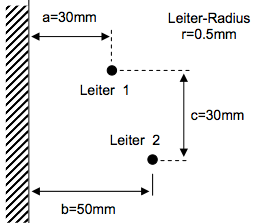
\includegraphics[width=3cm]{../El4/bilder/LeitungenParallel.png}
			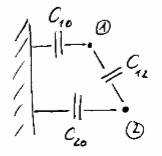
\includegraphics[width=3cm]{../El4/bilder/LeitungenKapazitaeten.png} \\
			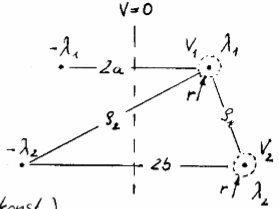
\includegraphics[width=5cm]{../El4/bilder/LeitungenParallel2.png}
		\end{tabular}
	\end{minipage}
 
		
\subsection{Induktivitätsbelag}
	\begin{tabular}{ll}
    	\begin{minipage}{12cm}
			\renewcommand{\arraystretch}{1.1}
				\begin{tabular}{| l | l |}
					\hline
						\textbf{Rotation B-Feld}
						& $\vec{B}=rot\vec{A}$ \qquad $A(\varrho)=-\frac{\mu_0 I}{2\pi}ln(\frac{\varrho}{k})$\\
					\hline
						\textbf{Linienströme}
						& $+I \qquad -I$\\
					\hline
						\textbf{$\mu_0$}
						& $4\pi\cdot 10^{-7}[\frac{Vs}{Am}]$\\
					\hline
						$\begin{matrix}
                         	\textbf{Leiterpotentiale}\\
                         	(aus Beispiel)
                         \end{matrix}$
						& $\begin{matrix}
                           	A^{+}=\frac{\mu_0 I}{2\pi}(-ln\frac{r}{k}+ln\frac{\varrho_1}{k}-ln\frac{2a}{k}+ln\frac{\varrho_2}{k})=\frac{\mu_0 I}{2\pi}ln\frac{\varrho_1\varrho_2}{2ar}\\
                           	A^{-}=\frac{\mu_0 I}{2\pi}(-ln\frac{\varrho_1}{k}+ln\frac{r}{k}-ln\frac{\varrho_2}{k}+ln\frac{2b}{k})=-\frac{\mu_0 I}{2\pi}ln\frac{\varrho_1\varrho_2}{2br}
                           \end{matrix}$\\
					\hline
						\textbf{Äussere Induktivität}
						& $L_a=\frac{1}{I}(A^{+}-A^{-})=\frac{\mu_0}{2\pi}ln(\frac{\varrho_1^2 \varrho_2^2}{4r^2ab})$\\
					\hline
						\textbf{Innere Induktivität}
						& $L_i=\frac{\mu_0}{8\pi} \quad \text{pro Leiter}$\\
					\hline
						\textbf{Induktivitätsbelag}
						& $L'=L_a+2L_i=\frac{\mu_0}{\pi} (ln(\frac{\varrho_1 \varrho_2}{2r\sqrt{ab}})+\frac{1}{4})$\\
					\hline
				\end{tabular}
			\renewcommand{\arraystretch}{1}
		\end{minipage}
    \end{tabular}
	\begin{minipage}{6cm}
    	\begin{tabular}{ll}
	    	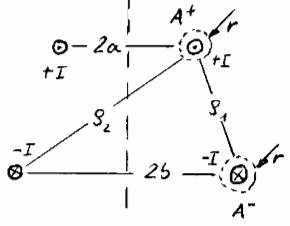
\includegraphics[width=5cm]{../El4/bilder/Induktivitaetsbelag.png}
		\end{tabular}
	\end{minipage}

\subsection{Stehende Wellen}
%	\subsubsection{Eigenschaften}
		\begin{tabular}{ll}
	    	\begin{minipage}{9cm}
				\renewcommand{\arraystretch}{1.1}
					\begin{tabular}{| l | l |}
						\hline
							\textbf{Spannung}
							& $|\underline{U}(z)|=|\underline{U}^+ e^{-j\beta z}(1+\underline{\Gamma}_L e^{2j\beta z})|=|\underline{U}^+| |1+\underline{\Gamma}_L e^{2j\beta z}|=|\underline{U}^+||1+|\underline{\Gamma}_L| e^{j(\Phi-2\beta z)}|$\\
						\hline
							\textbf{Strom}
							& $|\underline{I}(z)|=|\underline{U}^+ / \underline{Z}||1-|\underline{\Gamma}_L| e^{j(\Phi-2\beta z)}|$\\
						\hline
							\textbf{Spannungsmaxima bei:}
							& $e^{j(\Phi-2\beta z)}=1$\\
						\hline
							\textbf{Spannungsminima bei:}
							& $e^{j(\Phi-2\beta z)}=-1$\\
						\hline
					\end{tabular}
				\renewcommand{\arraystretch}{1}
			\end{minipage}
	    \end{tabular}

		\begin{tabular}{p{9cm}p{9cm}}
        	\begin{minipage}{8cm}
            	Spannungsbetrag mit kompl. Abschlussimpedanz:\\
            	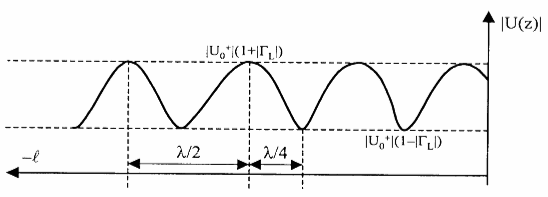
\includegraphics[height=2cm]{../El4/bilder/VerlaufSpannungsbetrag.png}
            \end{minipage}
			&
			\begin{minipage}{8cm}
            	Spannungs- Strombetrag der offenen Leitung:\\
            	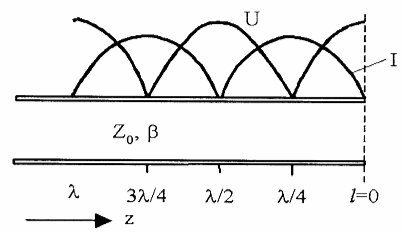
\includegraphics[height=2cm]{../El4/bilder/VerlaufSpannungsbetragOffeneLtg.png}
            \end{minipage}
        \end{tabular}
	
	\subsubsection{Spezialfälle}
		\textbf{Kurzschluss/Leerlauf}\\
			Bei Kurzschluss oder Leerlauf, also Reflexionsfaktor $\underline{\Gamma}$ ist -1 oder 1, verschwinden die Spannungs- Stromminima.
			Da die rückläufige Welle ebensoviel Energie transportiert wie die hinlaufende, wird längs der Leitung keine Energie transportiert.
			Es sieht also so aus, als ob die Welle am Ort stehen bleibt (Bild 2).\\
		\textbf{Leitung ideal abgeschlossen}\\
			Ist die Leitung ideal abgeschlossen, existiert keine reflektierende Welle.
			Die hinlaufende Welle transportiert so die gesammte Energie vom Sender zum Empfänger.\\
		\textbf{Leitung nicht ideal abgeschlossen}\\
			Es entsteht beim Empfänger eine Überlagerung der absorbierten und der stehenden Welle.
			Aus dem Verhältnis von Spannungsmaximum zu Spannungsminimum entsteht das Stehwellenverhältnis SWR.
			
			$$\text{Stehwellenverhältnis}: \quad SWR=\frac{U_{max}}{U_{min}}=\frac{1+|\Gamma_L|}{1-|\Gamma_L|} \qquad \text{Betrag des Reflexionsfaktor}:|\Gamma_L|=\frac{\text{SWR} -1}{\text{SWR} +1}$$

	\subsection{Mehrfachreflexion}
% 	\textbf{Lastseitig falsch abgeschlossen}\\
% 	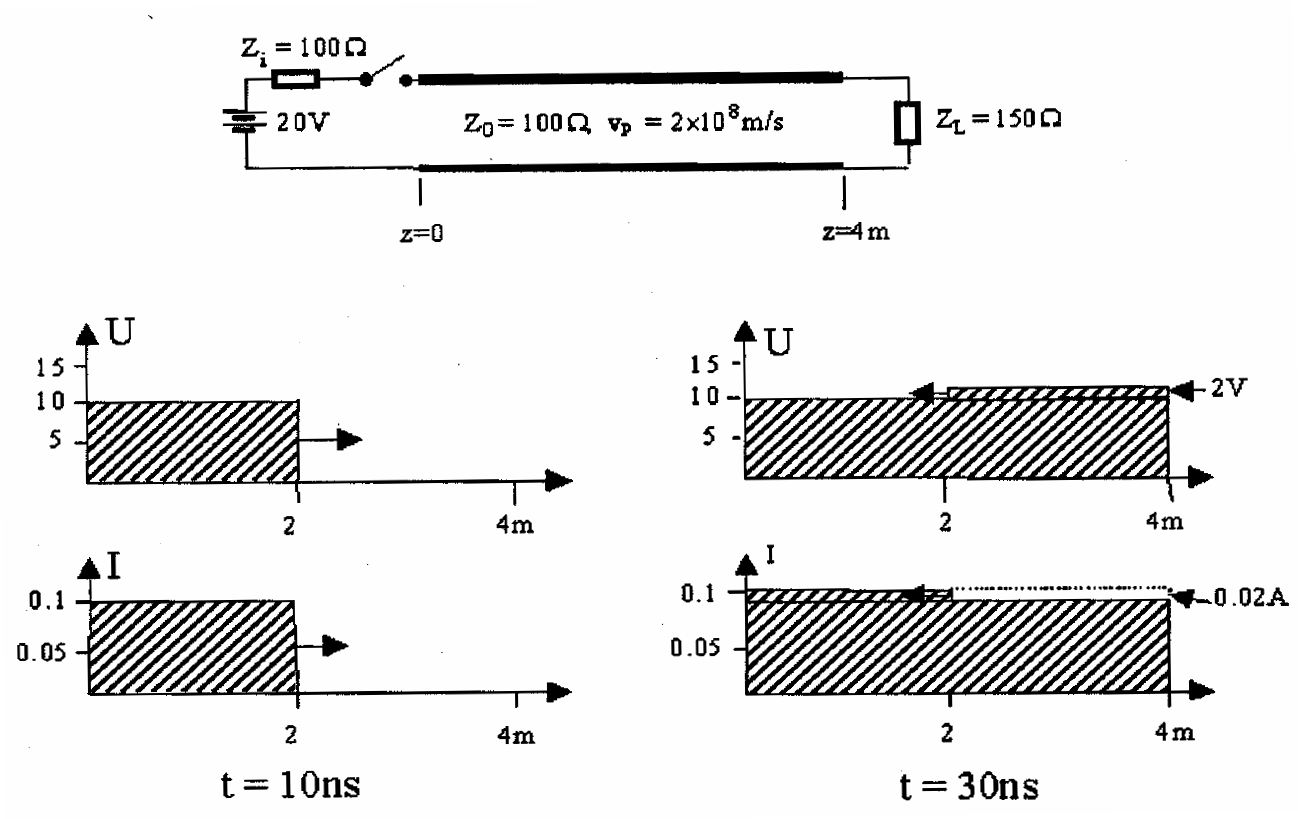
\includegraphics[height=3.5cm]{../El4/bilder/Leitungen_MFReflx_EnAP_SAP.png} \textbf{text folgt} \\
	\begin{tabular}{p{9cm}p{9cm}}
		\begin{minipage}{8cm}
			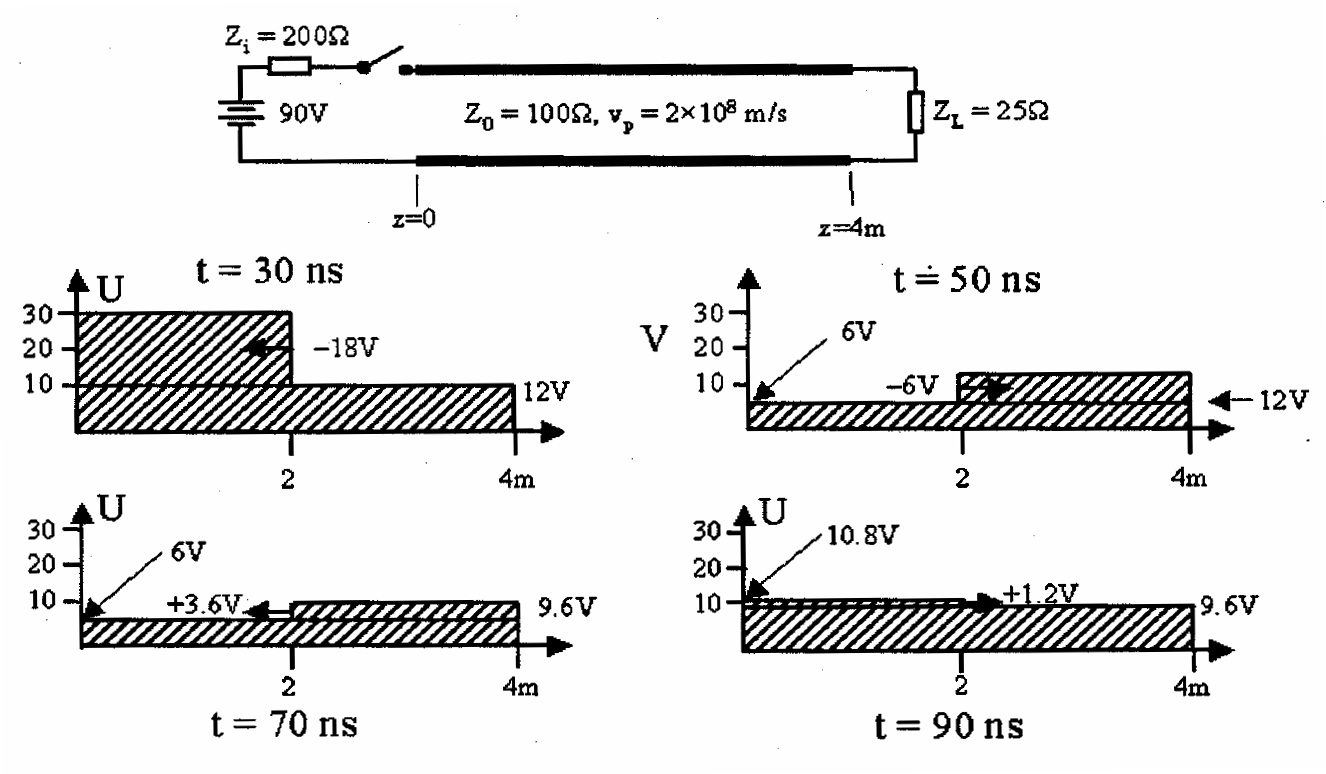
\includegraphics[width=8cm]{../El4/bilder/Leitungen_MFReflx_EnAP_SnAP.png}
	    \end{minipage}
		&
		\begin{minipage}{9cm} 	    	
    		Das nebenstehende Schema zeigt eine Leitung, welche last- und quellenseitig falsch
    		abgeschlossen ist. \\
    		Zur Berechnung der Spannung $\underline{U}_{0}^+$ werden alle Widerstände am Leitungsende
    		ignoriert ($\underline{Z}_L = 0$).
    		Die reflektierenden Wellen werden anhand der Reflexionskoeffizienten
    		$\underline{\Gamma}_{Last}, \underline{\Gamma}_{Quelle}$ berechnet. Bsp.:
    		\\ \\
    		$\underline{U}_{0}^+ = \frac{U_{Quelle} \underline{Z}_0}{ \underline{Z}_0 +
    		\underline{Z}_i}; \quad \underline{U}_{0}^- = \underline{U}_{0}^+ \cdot 
    		\underline{\Gamma}_{Last}; \\ \underline{U}_{1}^+ = \underline{U}_{0}^- \cdot 
    		\underline{\Gamma}_{Quelle}; \quad
    		\underline{U}_{1}^- = \underline{U}_{1}^+ \cdot 
    		\underline{\Gamma}_{Last}; \quad$ usw.   \\ 
    		$\underline{U}_{Resultierend} = \underline{U}_{0}^+ + \underline{U}_{0}^- +
    		\underline{U}_{1}^+ + \underline{U}_{1}^- +  \ldots  + \underline{U}_{n}^+ +
    		\underline{U}_{n}^-$
	    \end{minipage}  
		\\
		\begin{minipage}{8cm}  
			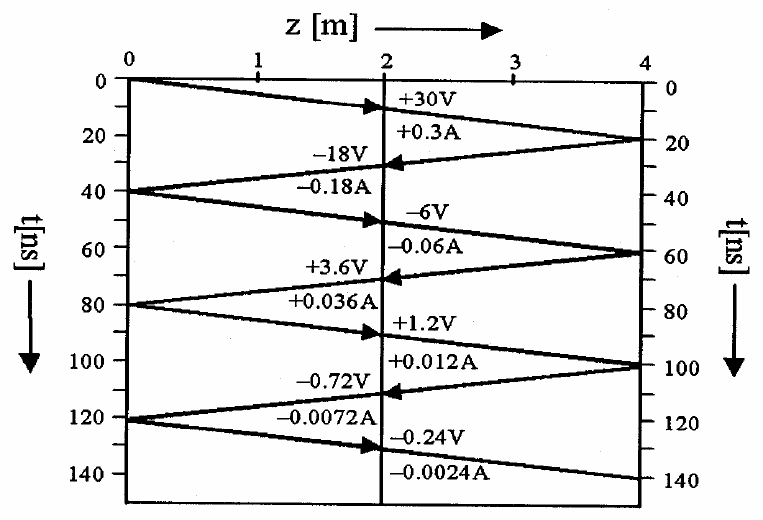
\includegraphics[height=4.1cm]{../El4/bilder/Leitungen_MFReflx_EnAP_SnAP_RaumZeit.png}    	    
	    \end{minipage}
		&
		\begin{minipage}{8cm}
			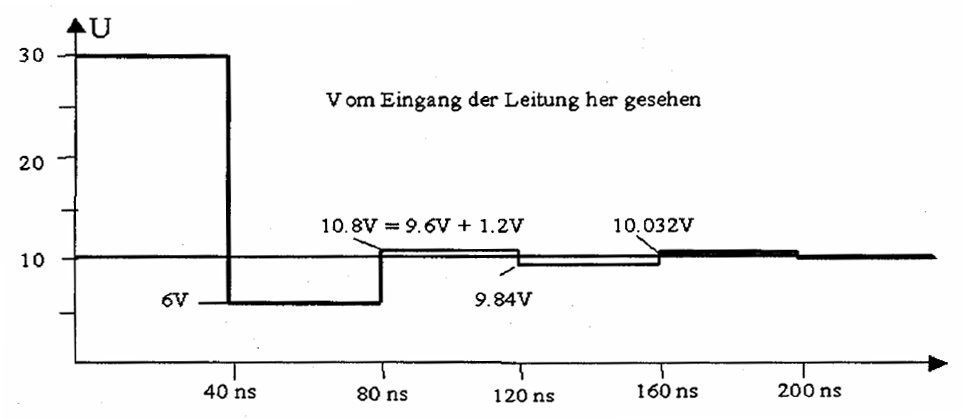
\includegraphics[height=4.1cm]{../El4/bilder/Leitungen_MFReflx_EnAP_SnAP_Eingangsspannung.png}      	
	    \end{minipage}
	\end{tabular}

    